\documentclass[../manuscript.tex]{subfiles}

\section{Введение}

Секвенирование одиночных клеток на протяжении последних нескольких лет было одной из самых горячих тем в науке: single-cell технологии дважды получали звание "method of the year" по версии Nature Methods\cite{MethodOfTheYear2013, MethodOfTheYear2019}, а 10X Genomics, основная компания-производитель оборудования для single-cell секвенирования, заняла 69 строчку в рейтинге 500 наиболее быстрорастущих компаний США\footnote{https://www.inc.com/inc5000/2019/top-private-companies-2019-inc5000.html}. Возможность изучать биологические процессы в тканях на уровне отдельных клеток привела к прорывным открытиям во многих областях науки\cite{SingleCellRevolution, SingleCellComingOfAge}, особенно в персонализированной онкологии\footnote{https://www.nature.com/articles/d42473-019-00310-5}. В частности, в задаче восстановления клональной структуры опухоли — определения групп клеток, имеющих схожий набор индуцированных генетических мутаций. Понимать состав опухоли критически важно для подбора лечения, особенно в высокоинвазивных раках с высокой частотой мутаций. 

\begin{figure}[H]
	\centering
	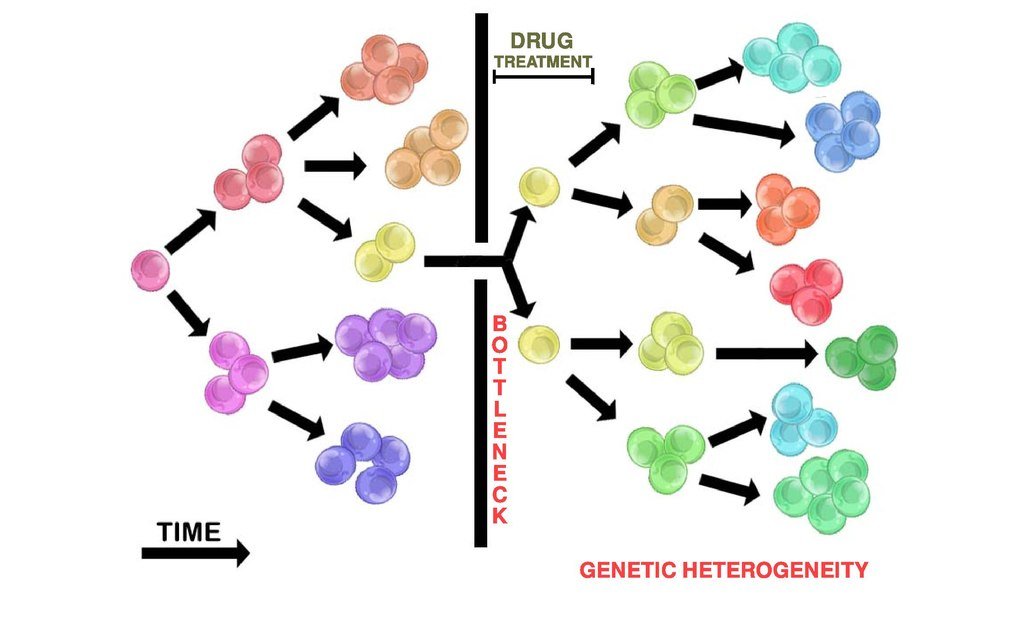
\includegraphics[keepaspectratio=true, scale=0.4]{images/tumour_heterogeneity_treatment_bottleneck.jpg}
	\caption{При подборе терапии нужно учитывать клональный состав опухоли. Лечение может убивать некоторые клональные линии, но не действовать на остальные, из-за чего случается рецидив.}
\end{figure}

В данной дипломной работе рассматривается байесовский подход к этой задаче, которую называют одной из 11 главных задач вычислительной биологии одиночных клеток\cite{ElevenGrandChallengesInSingleCellDS}. В работе предложены две версии алгоритма байесовского машинного обучения XClone — графической модели опухоли. В задачи XClone входит не только анализ клонального состава образца, но и поиск аллель-специфических структурных мутаций, по которым можно пронаблюдать эволюцию опухоли. Алгоритм XClone развивает идеи, заложенные доктором Янхуа Хуань в статьях "Cardelino"\cite{Cardelino} и "Vireo"\cite{Vireo}. 

Текущая  версия XClone состоит из двух основных частей, связанных расстановкой клональных меток. 

Первая часть получила название "RDR-модуль", где RDR расшифровывается как "read depth ratio", отношение наблюдаемой доли числа прочтений внутри фиксированного сегмента генома к ожидаемой. В теоретических моделях ДНК-секвенирования, где предполагается равномерное распределение прочтений по геному, RDR должно стремиться к реальному числу копий этого сегмента пополам. Это основная величина, на которую опираются алгоритмы поиска структурных вариаций генома, в том числе CellRanger от 10X Genomics и CHISEL\cite{ChiselBiorxiv}. В процессе работы над текстом ВКР стало ясно, что изначальная модель RDR-модуля не совсем точна. Это позволило разработать третью версию XClone, о которой идёт речь в заключительном разделе ВКР. Она будет реализована в ходе дальнейшей научной работы.

Вторая часть носит название "BAF-модуль", где BAF означает "B-allele frequency". Эта часть модели позволяет не только понять, сколько копий сегмента образовалось в процессе онкогенеза, но и сколько из этих копий лежит на каждой конкретной хромосоме. Важность этой информации была обоснова во многих статьях по онкологии. \cite{Zack2013, Pleasance2010, Waddell2015, Dentro312041}. К примеру, такая утрата гетерозиготности, при которой один аллель утерян, а второй дуплицирован, из-за чего суммарное число копий остаётся равным двум, характена для многих видов рака \cite{Pleasance2010, Thiagalingam2698, Langdon2006, Lapunzina2011}. Аллель-специфические структурные вариации также важны для детектирования дупликации генома \cite{Carter2012} и для уточнения момента в эволюции опухоли, когда дупликация произошла\cite{Zack2013, Carter2012, Gerstung2020}. Несмотря на это, в более ранних методах считалось, что данные single-cell секвенирования слишком разреженные для их определения \cite{Zahn2017, Laks411058}. Существующие методы, кроме CHISEL\cite{ChiselBiorxiv}, способны определять только число копий посредством анализа RDR. Стандартной техникой определения аллельного дисбаланса по данным bulk-секвенирования является анализ частоты гетерозиготных аллелей. Ранее считалось, что по данным single-cell секвенирования эти частоты надёжно определить нельзя, но и XClone, и CHISEL демонстрируют, что это возможно.

По состоянию на июнь 2020 года, опубликован только один непосредственный аналог XClone — алгоритм CHISEL\cite{ChiselBiorxiv}, разработанный в лаборатории Бена Рафаэля в Принстонском университете. CHISEL был выложен на онлайн-архив предпубликаций bioRxiv уже после того, как была начата работа над XClone. Тем не менее, несмотря на то, что оба метода дают сравнимые результаты в задаче поиска аллель-специфических структурных вариаций, XClone выгодно отличается от CHISEL тем, что в его статистическую модель можно естественным образом интегрировать другие типы данных, такие как данные РНК-секвенирования, данные о соматических мутациях, данные о митохондриальной ДНК, в то время как алгоритм CHISEL решает узкую задачу и никаким тривиальным образом не обобщается. Авторы верят, что именно в этой гибкости и масштабируемости заключается научная новизна XClone.

Метод был опробован на реальных данных, извлечённых из медуллобластомы — детской опухоли мозга, — полученных по протоколам компаний 10X Genomics\footnote{https://www.10xgenomics.com/products/single-cell-cnv/} и Smart-Seq\footnote{https://www.illumina.com/science/sequencing-method-explorer/kits-and-arrays/smart-seq2.html}, но концептуально он не привязан к конкретной платформе и может быть адаптирован к другим форматам входных данных.

На концептуальном уровне, XClone также можно использовать для интеграции геномных и транскриптомных данных, но на данный момент, в силу низкого разрешения данных РНК-секвенирования одиночных клеток, эту гипотезу не удаётся убедительно доказать. Кроме того, в процессе работы над алгоритмом, к сожалению, стало ясно, что опухоль в образцах медуллобластомы однородная: в ней выжила всего одна клональная линия. Тем не менее, авторы ведут переговоры с научной группой из Стэнфорда, располагающей более удачными образцами опухоли желудка. По предварительным сведениям, их образцы содержат порядка 10 отчётливо различимых клональных линий, а глубина покрытия должна позволить получить приемлемое отношение сигнала к шуму. 

Специфика предметной области определила не совсем обычную для статей по машинному обучению структуру экспериментов в данной ВКР: каждая опухоль индивидуальна, а секвенирование стоит больших денег, потому как таковой обучающей выборки не было. Даже генерация синтетических данных это отдельная нетривиальная задача, которая до сих пор не решена на должном уровне. Более того, в момент начала работы метод не имел аналогов, потому статистическая модель приобрела свой нынешний вид методом проб и ошибок. 

Даже сравнить методы и доказать, что один из них лучше другого, на данный момент возможно только на качественном уровне, т.к. по состоянию на 2020 год просто нет реальных данных, в которых в каждой из клеток были бы достоверно известны все структурные вариации генома. Масштабные же вариации хорошо предсказывает как XClone, так и CHISEL. Тем не менее, ведётся активная разработка более продвинутой генерации синтетических клеток. Как только она будет завершена, оба метода будут подвергнуты тщательному сравнительному анализу.

Но несмотря на все эти трудности всего за полгода был получен значительный прогресс. Есть основания рассчитывать на публикацию улучшенной версии алгоритма XClone в высокоимпактных журналах: алгоритм Cardelino\cite{Cardelino}, на котором была основана первая версия XClone, в марте 2020 года был опубликован в Nature Methods. 